 \section{Inpainting}
 %MODIFIER ICI
\begin{frame}
  \frametitle{Inpainting :D}
  \begin{itemize}
  \item FAIRE UNE DIAPO DE SECTION SERAIT MIEUX !!
  \end{itemize}

\end{frame}



 %%%%%%%%%%%%%%%
 % Frame Architecture inpainting
\begin{frame}
  \frametitle{Architecture du programme}
  \insertF{Fig/architectureInpainting.png}{Architecture de la partie Inpainting}{1}


\end{frame}



 %%%%%%%%%%%%%%%
 % Frame KeyPoints
\begin{frame}
  \frametitle{Keypoints}
  
  \begin{itemize}
  \item SURF
  	\begin{itemize}
  	\item
  	\end{itemize}
  	
  \item GFTT (Harris)
	\begin{itemize}
  	\item
  	\end{itemize}
  	
  \item Canny
    \begin{itemize}
  	\item
  	\end{itemize}
  	
  \end{itemize}
    \insertF{Fig/cannyPoints.png}{Points de Canny}{0.4}


\end{frame}



 %%%%%%%%%%%%%%%
 % Frame create trace
\begin{frame}
  \frametitle{Trace}
  \begin{itemize}
  \item Recherche de correspondances entre points
  	\begin{itemize}
  	\item Sélection des keypoints
  	\item Recherche dans le voisinage frame suivante
  	\end{itemize}
  \item Estimer l'homographie
  \item Trace
  	\begin{itemize}
  	\item Créer et continuer la trace
  	\item Classifier la trace
  	\begin{itemize}
  		\item fixe
  		\item mobile
  		\item indéterminé
  	\end{itemize}
  	\end{itemize}
  \end{itemize}
  
    \insertF{Fig/cannyKeypoints.png}{Mise en évidence des keypoints et de la trace}{0.4}


\end{frame}


 %%%%%%%%%%%%%%%
 % Frame inpainting principe
\begin{frame}
  \frametitle{Remplissage}
  
  \begin{itemize}
  \item Classifier les zones
  	\begin{itemize}
  	\item fixe $\leftrightarrow$ noir
  	\item mobile $\leftrightarrow$ couleur du fond
  	\end{itemize}
  \item Remplir quand le point devient fixe  
  \end{itemize}

  \begin{figure}
  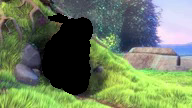
\includegraphics[width=0.45\textwidth]{Fig/bunny2-masked.png}
  
\includegraphics[width=0.45\textwidth]{Fig/bunny1-original.png}
  \caption{Principe de l'inpainting 2D + t}
  \end{figure}
   
\end{frame}


 %%%%%%%%%%%%%%%
  % Frame demonstration
 \begin{frame}
   \frametitle{Démonstration}
   \insertF{Fig/workInProgress.png}{Lancement de la démonstration inpainting 2D + t}{0.5}


 \end{frame}